\chapter{Synthetic geophysical test}

This chapter will outline a series of experiments which will test the main postulate of this thesis, that ABC can offer some improvement over traditional likelihood based Bayesian inference for geophysics. There are many potential avenues to pursue 'improvement'. For example, ABC opens parameter inference to models which were previously closed. This can be used to compare the solution of parameter inference for a stochastic forward where the data and modelization uncertainty do not conform to a Gaussian, to the solution obtained with the simplifying assumption that the uncertainty is Gaussian. This may constitute an improvement in accuracy if it is shown that the ABC solution is significantly different from the analytical Gaussian solution. Instead of pursuing this angle, here I focus explicitly on improving the speed of optimization relative to a general form MCMC sampler. Probabilistic methods which rely on Monte Carlo and MCMC are computationally expensive due to the need to compute the forward at every iteration of the algorithm. As a result the scale of the problems which are computationally tractable is limited. If our limits of understanding about the Earth are to be pushed then it is necessary to develop methods which can tackle large scale problems which are fundamentally defined by solution spaces with uncertainty due to trade-offs between parameters, uncertainty in the experimental data and uncertainty in the modelization process. In this context there is great need for methods which can efficiently find, and then define regions of high probability in very sparse parameter spaces. \par

Here I seek to use the information available by 'opening' the likelihood within each forward simulation to drive improved optimization with ABC, a method which can take into account the full scope of uncertainty in the resulting solution. In this way I abandon the mathematical generality of the applied sampling algorithm in pursuit of one purpose built for the information available within the problem. \par

As with the previous chapter, the code to produce all figures in this section can be found at \url{https://github.com/tomconnell/approximate-bayesian-tomography}.\par


\section{Crustal density inversion}

As a first experiment, I consider an inversion for crustal density (\rho) with a vertical gravity anomaly dataset (\Delta g) for a 2D discretized subsurface \citep[p.184-195,378]{blakely1996}. The dimensionality of the parameter space is kept modest, a 8x4 grid, with an observed data point above each column. The grid is defined over a 160 $km$ by 40 $km$ area. The parameter space is bounded between 2-3.5 $g/cm^3$, the limits for which \citet{Brocher2005} define an empirical relationship between density and compressional-wave velocity ($V_p$). This relationship will be used in the next section for a joint inversion. The 'true model', which will be the target of our inversion scheme, is kept smooth to allow a prior term, $p(\bm{\theta})$, to be set for smoothness which will limit the inversion to a unique solution. The definition for smoothness is:
\begin{equation}
\text{log}\big(p(\bm{\theta})\big) = \sum_{i = 1}^{N} \Big(\sum_{j} (\rho_i - \rho_j)^2\Big)
\label{smoothness}
\end{equation}
where $j$ is a describes all blocks in immediate contact with the given block, $i$. The edge effect for the 2D subsurface grid is compensated by adding the vertical gravity anomaly which will result from extending the grid by a width of one on both sides, tripling the total domain width, with a density which is the average of the parameter space, 2.75 $g/cm^3$. The model is assumed to contain no modelization uncertainty and the data is known to be contaminated with noise defined by $\sigma^{\mathcal{D}} = \mathcal{N}(0,\sqrt{2})$.
\begin{figure}[H]
	\centering
	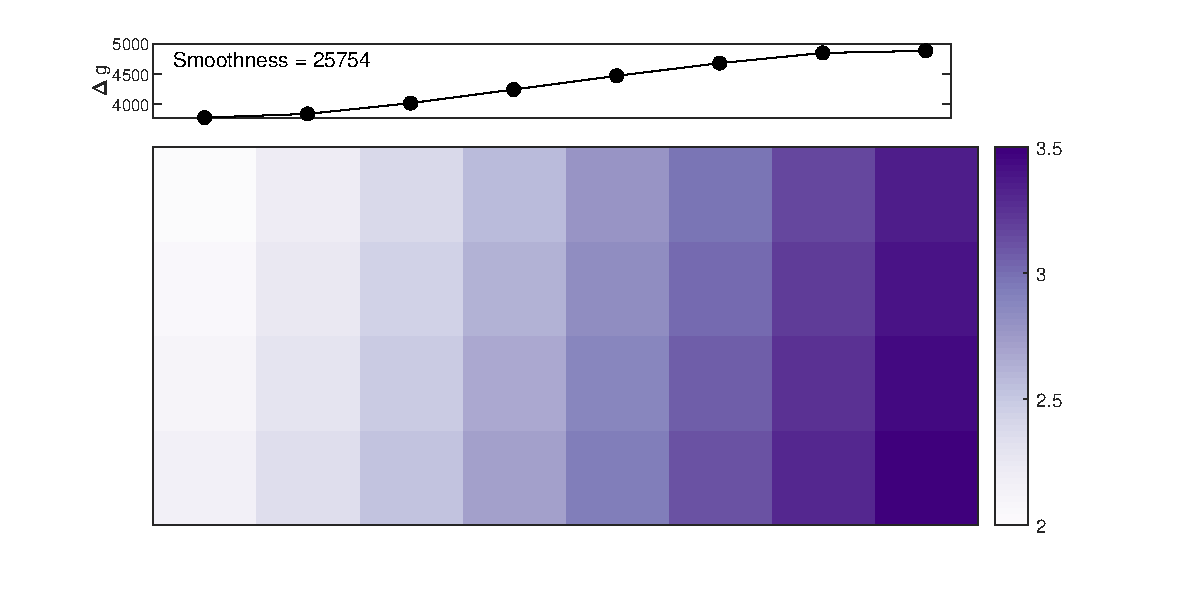
\includegraphics[scale=0.8]{true_model.pdf}
	\caption{The 'observed data', vertical component of gravity ($\Delta g$), and 'true model', a 2D density ($g/cm^3$) slice, which will be the target of our synthetic geophysical experiments to compare ABC to likelihood based Bayesian inference. A smoothness value, log($p(\bm{\theta})$), equation \ref{smoothness}, for the true model is plotted for reference to later solutions.}
	\label{true_model}
\end{figure}
The benchmark for ABC-tomography to meet will be MCMC sampling of an analytically defined posterior. Given there is no modelization uncertainty and $\sigma^{\mathcal{D}}$ is known, the log-likelihood can be defined by, equation \ref{likelihood-1}:
\begin{equation}
	l(\bm{\theta^*}|\bm{y}) = \frac{(\bm{y}-\bm{y^*})^2}{(\sigma^{\mathcal{D}})^2}
\end{equation}
For this section only MCMC is considered, no AM, DR or DRAM. This maintains a consistent sampling benchmark for comparison to the ABC scheme. The proposal distribution for both MCMC sampling of the analytical distribution and ABC-tomography is held constant for all runs as $q(\cdot,\cdot) = \mathcal{N}(0,I\cdot250)$. The parameter space is subdivided into eight 2x2 blocks. At each time step a random block is selected in the subsurface and updated via $q(\cdot,\cdot)$. As demonstrated in table \ref{sampling-method-comparison}, the number of parameters updated at each time step impacts the acceptance rate and the rate of space exploration of the chain. To keep inference comparable both the analytical scheme and ABC scheme will update 4 parameters per time step via the proposal distribution. Likewise, for each experiment considered in this section the Markov chain starting position is the same for both the analytical and ABC-tomography. The starting position for both is set by sampling a uniform distribution, $\mathcal{U}(2,3.5)$, to define each unknown parameter. \par
A set of summary statistics to describe the data in Figure \ref{true_model} is needed to proceed with ABC-tomography. Here I seek safety in a comprehensive description of the data by the co-efficients to a linear model, $m$ and $b$, the sample mean, $\bar{\mu_{\Delta g}}$, sample standard deviation, $\bar{\sigma_{\Delta g}}$, and a failsafe residual term, $\sum R$, for the difference between a simulation and the observed data for a given $\bm{\theta^*}$, $R = |\bm{y}-\bm{y^*}|$. Initial testing showed the set of statistics $\begin{bmatrix}
\bar{\mu_{\Delta g}}\ \bar{\sigma_{\Delta g}}\ m\ b\ \sum R
\end{bmatrix}^T$ comprehensively describes $\bm{y}$. As with section \ref{banana-section}, it is necessary to normalize the spread of each marginal distance term, $\text{d}_i(S_i(\bm{y}),S_i(\bm{y^*}))$, equation \ref{marginal_distance}, to one. This accounts for the different scales and sensitivities of the summary statistics to the unknown parameters. The normalization term $\bm{\sigma_S}$ is approximated from >10,000 Monte Carlo simulations over parameter range 2-3.5 $g/cm^3$. The tolerance is closely related to the acceptance rate of the algorithm. The tolerance is tuned to give reasonable acceptance rate (approx. 20\%).\par
For the ABC-tomography scheme I am free to open the likelihood, consider the information available, and use that to drive the next step in the Markov chain. As a first adjustment I localize the updates to directly below a data point, and choose which column of parameters to transition based on a probability distribution proportional to the misfit between the observed data $\bm{y}$, and the simulated data set $\bm{y^*}$. Here and throughout misfit is defined by the l2-norm:
\begin{equation}
	\text{misfit} = (\bm{y}-\bm{y^*})^2
\end{equation}
The effectiveness of dynamically selecting and localizing the updates relies on our physical intuition about the relationship between the unknown model parameters and the resulting data. In this case the simulated data is most sensitive to the blocks which are directly below, and by focusing model updates on regions which are poorly fitting, the most is made from each move during the initial optimization phase in finding areas of high posterior probability density. This change has ideas similar to the way gradient-based linear optimization methods work, however, here I simply rely on physical intuition. \par
Figure XX plots a comparison between the analytical scheme described above and ABC-tomography during the optimization phase of the respective Markov chains (first 10,000 time steps). Figure YY and ZZ plot the solution obtained, mean marginal model, for the full chain (YY time steps). Figure AA and BB plot the chain trace and posterior density for select parameters. 



\citet{Sisson2010a} highlight that sampler acceptance rate and mixing can be improved by increasing the number of simulated datasets, $\bm{y^*}$, for each set of model parameters, $\bm{\theta^*}$. This is a technique also adopted in applications with large uncertainty in $\bm{g_s}$ \citep{Ratmann2009,Wood2010}. This has a large stabilizing impact when the uncertainty in each simulation is large. Here I adopt this technique for $k = 100$ simulations from $\bm{g_s}$. Since the bulk of the computational overhead is in solving the deterministic physical model and the data uncertainty is additive and fast to simulate, there is little computational cost in increasing  the number of simulated datasets. The distance is then computed based the sample mean of $\bm{y^*_{1:k}}$, $\bm{d} = |\bm{S}(\bm{y})-\bm{S}(\bm{\bar{\mu_{y^*}}})|$.



\section{Crustal density joint inversion}